\section{Framework}
\label{sec:framework}

Our framework has four main components: Path generation, Path searching, Schedule and Transport as depicted in Figure \ref{fig:framework}.

\begin{figure}[!htb]
\vspace{-0.1in}
\centering
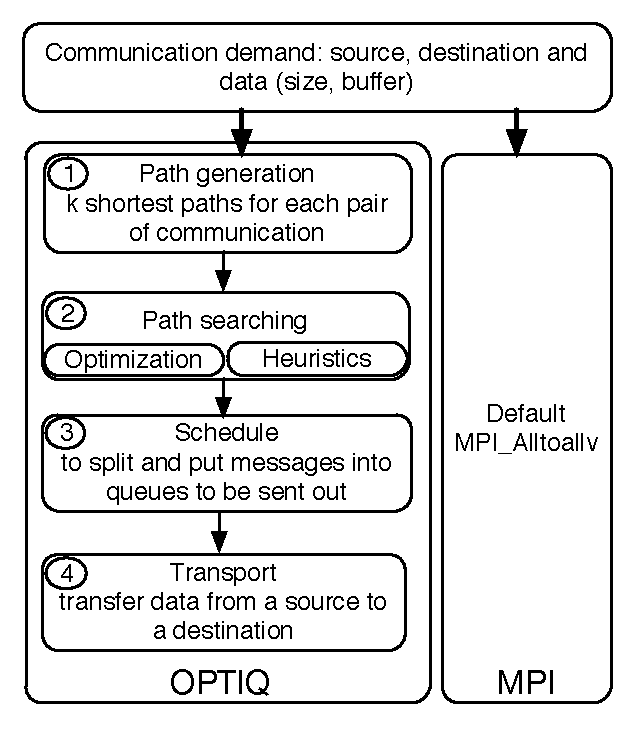
\includegraphics[scale=0.7]{figures/framework.pdf}
\vspace{-0.1in}
\caption{Four components of OPTIQ framework}
\vspace{-0.1in}
\label{fig:framework}
\end{figure}

The functionality of each component is as follows:
\begin{itemize}
\item Path generation: generate k shortest paths that can be used as candidates for data tranfser. We need to generate paths to reduce the search space.
\item Path searching: search for paths to transfer data from a set of sources to a set of destinations. Multiple paths or a single path can be found using a set of approaches. User can use one of the approaches provided by the framework or can add their own approaches.

\item Schedule: Split a buffer of data that needs to be tranferred into smaller messages and put those messages into a queue of the Transport layer to be transferred. It also handles the order of sending and forwarding messages.

\item Transport: actually transfer an amount of data from one point to another point in the system.

\end{itemize}

The framework has various options to allow users to tune the framework for optimal performance, such as order of sending or forwarding messages, choosing path searching algorithms, setting chunk size to transfer messages. 
